\subsection{Vergleich der Algorithmen}
Die Algorithmen werden in Abbildung \ref{fig_euklid_dijkstra_fast_marching_vergleich} in Vergleich gesetzt. Dafür wird eine Karte erstellt mit einem Raum, einer Tür und einem Hindernis vor der Tür. Die Karten werden jeweils nach 1, 20, 100, 1000 Schritten geplottet. Als letztes wird noch das Gesamtergebnis dargestellt.

\subsubsection{Euklid}
Um den Euklidischen Abstand zu berechnen, benötigt man lediglich die Position des Ziels, die Position der aktuellen Zelle und die Zellbreite. Man geht alle Zellen der Reihe nach durch und berechnet den Abstand der aktuellen Zelle zum Ziel. Die Suche nach noch nicht berechneten Zellen läuft nicht von oben nach unten sondern mit der Funktion \glqq parallelStream()\grqq . Diese teilt das Feld in Teilfelder auf und sucht parallel nach freien (noch nicht berechneten) Feldern. Dadurch entstehen die in Abbildung \ref{fig_euklid_dijkstra_fast_marching_vergleich} sichtbaren Stufen. \cite{JavaParallelism} Darüber hinaus ist zu erkennen, dass das Hindernis vor der Tür für den Euklid Algorithmus keinen Einfluss hat. Dieses Hindernis wird bei der Berechnung ignoriert.

\subsubsection{Dijkstra}
Beim Dijkstra Algorithmus geht man ausgehend vom Ziel immer ein Feld weiter und berechnet den Abstand des aktuellen Feldes anhand des Abstand des Nachbarfeldes. Dadurch wird die Karte ausgehend vom Ziel aufgebaut wie in Abbildung \ref{fig_euklid_dijkstra_fast_marching_vergleich} zu sehen ist. Es ist auch zu erkennen, dass der Dijkstra Algorithmus die Abstände um das Hindernis berechnet. Das Hindernis wird also in die Berechnung einbezogen.

\subsubsection{Fast Marching}
Ähnlich wie beim Dijkstra arbeitet der Fast Marching Algorithmus vom Ziel aus. Das Zielfeld wird als Basis angenommen und die Nachbarfelder um das Ziel werden als \glqq considered\grqq  also als \glqq in Betracht kommend\grqq  markiert. Das in Betracht kommende Nachbarfeld mit dem besten Wert wird als \glqq accepted\grqq  also als \glqq akzeptiert\grqq  markiert. Danach wird für alle Nachbarn dieses akzeptieren Feldes die Entfernung mittels der Eikonalgleichung berechnet. Auch hier ist also die Berechnung abhängig von den vorher berechneten Feldern. Es ist deutlich zu erkennen, dass der Fast Marching Algorithmus eine deutlich rundere Karte erzeugt, als der Dijkstra.

\begin{figure}
\centering
\begin{minipage}{0.32\textwidth}
\centering
  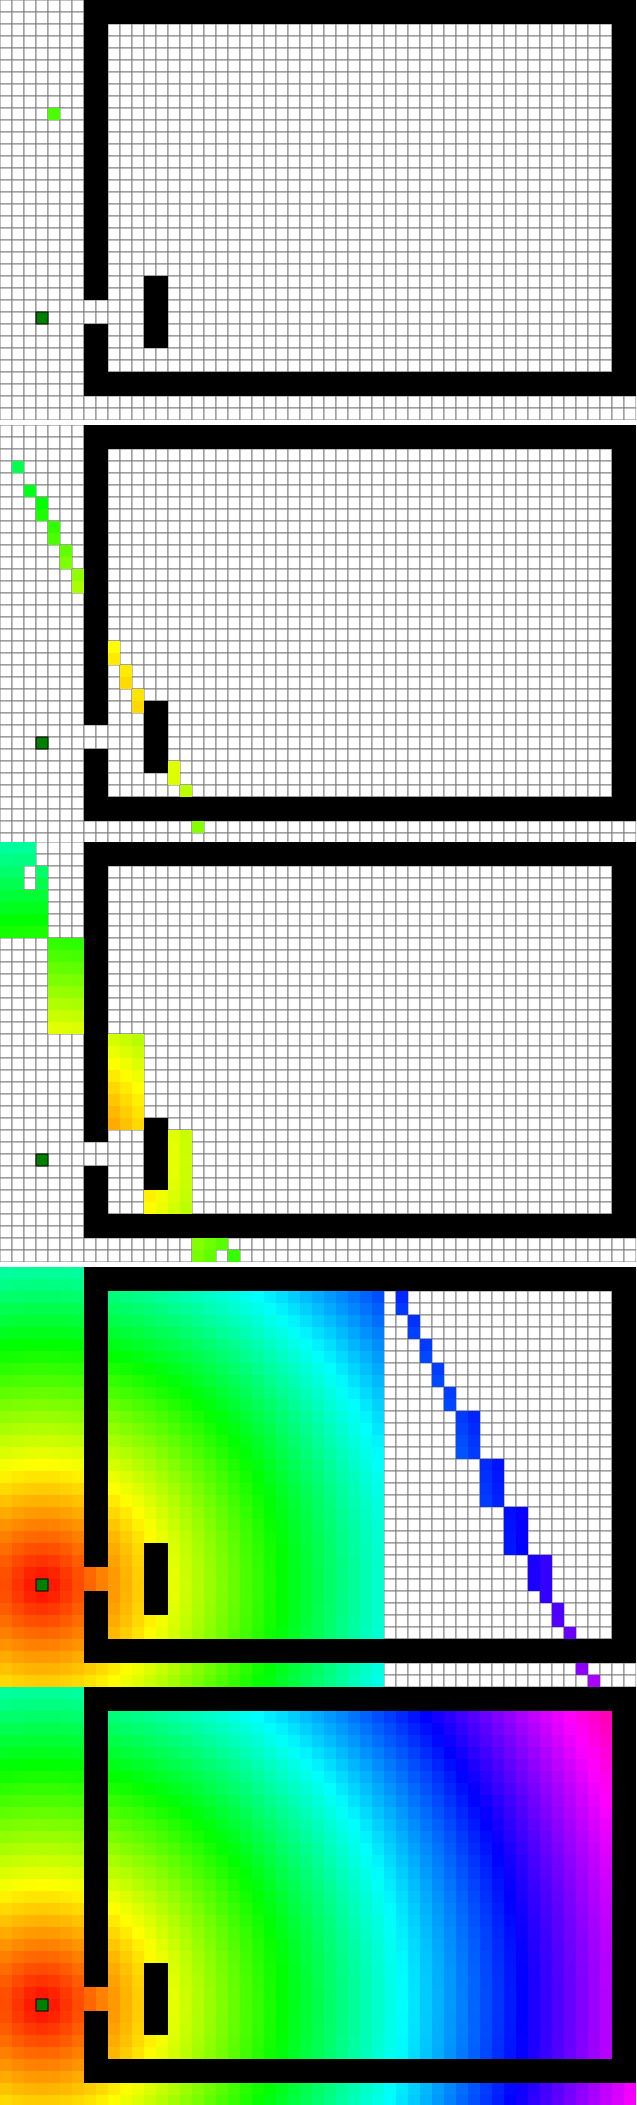
\includegraphics[width=\linewidth]{abbildungen/vergleich_euklid_fast_marching/snapshot_eEuclid_zusammen_cutted.png}
\end{minipage}%
\begin{minipage}{0.32\textwidth}
\centering
  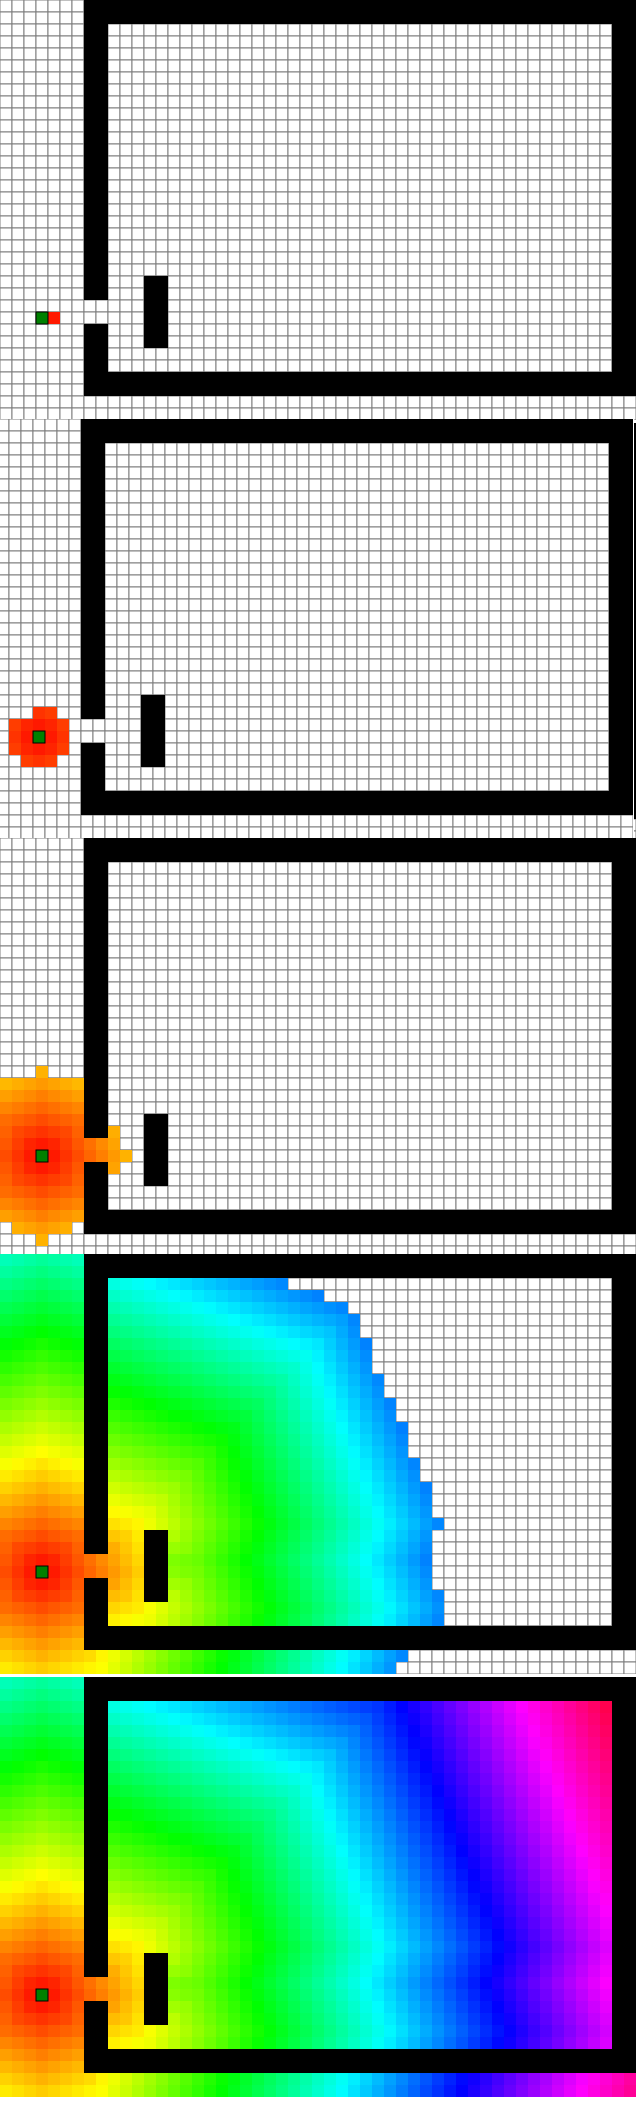
\includegraphics[width=\linewidth]{abbildungen/vergleich_euklid_fast_marching/snapshot_eDijkstra_zusammen_cutted.png}
\end{minipage}
\begin{minipage}{0.32\textwidth}
\centering
  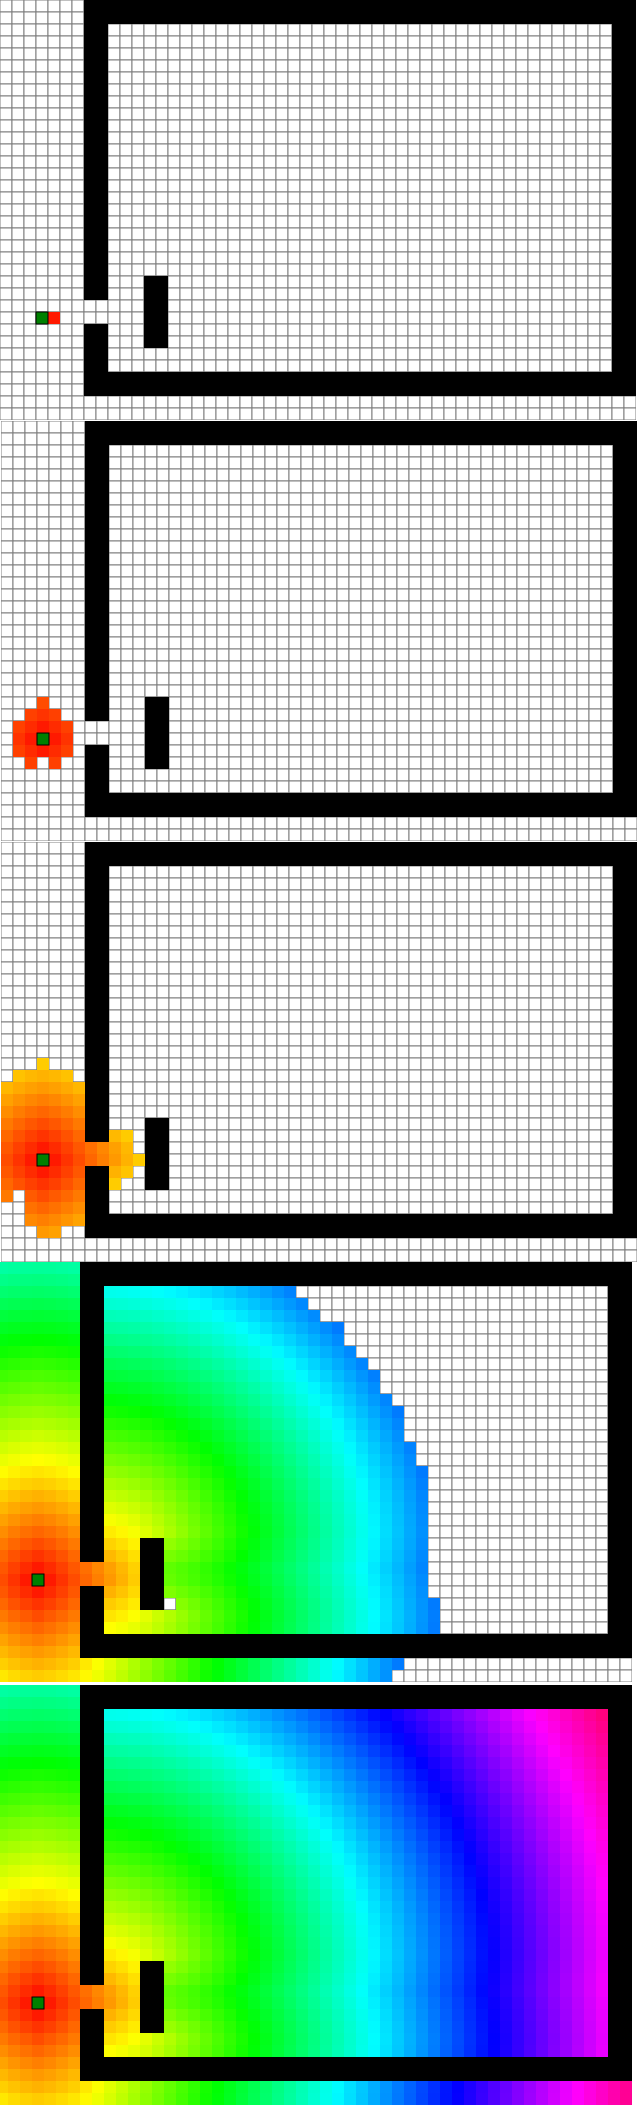
\includegraphics[width=\linewidth]{abbildungen/vergleich_euklid_fast_marching/snapshot_eFastMarching_zusammen_cutted.png}
\end{minipage}
\caption{Die berechnung der Abstände mit verschiedenen Algorithmen im Vergleich. Euklid (links), Dijkstra (mitte), Fast Marching (rechts), jeweils von oben nach unten nach 1, 20, 100, 1000 Schritten und Gesamtbild}
\label{fig_euklid_dijkstra_fast_marching_vergleich}
\end{figure}



\subsubsection{Einfluss der Zellgröße auf die Abstandsberechnung}
Bei der Berechnung der Abstände hat die Wahl der Zellgröße je nach Algorithmus einen entscheidenden Einfluss auf die Ergebnisse der Simulation. Die Zellgröße gibt nicht nur die minimale Schrittweite vor, sondern hat auch Einfluss auf die Genauigkeit der Nutzenberechnungen. An dieser Stelle wird der Euklid Algorithmus dem Fast Marching Algorithmus gegenübergestellt. Um einen Vergleich darzustellen wurde ein Quadratisches Feld angelegt. Die Zellgröße des Feldes sowie die Anzahl der Felder wurden so variiert, dass die Entfernung von der rechten unteren Ecke zur linken oberen Ecke (am weitesten entfernter Punkt) immer den gleichen Abstand hat. Es wird also die Diagonale des Rechtecks berechnet. 

\paragraph{Grafische Überprüfung}\\
Die Abbildung \ref{fig_euklid_fast_marching_2m_cellsize} Zeigt den Vergleich beider Algorithmen bei der der Abstandsberechnung. Üblicherweise wird die Farbskala so gewählt um alle Werte vom kleinsten Abstand zum weitesten Punkt abzubilden. Um den Vergleich an dieser Stelle deutlich zu machen, wurde für beide Bilder die selbe Farbskala verwendet. Mit Bloßem Auge ist die Differenz nur schwer zu erkennen. Es ist jedoch sichtbar, dass das Feld, welches mit dem Euklid Algorithmus berechnet wurde, einen deutlicheren Bogen aufweist. 

Eine Möglichkeit die Unterschiede zu visualisieren ist es, die Bilder mittels einer Differenzbildung der Beiden Bilder. Dafür wird ein Bild als Basis hergenommen und das zweite Bild als eine Ebene darüber eingefügt. Die Farben der zweiten Ebene werden von der ersten Ebene Subtrahiert. Gleichen sich die Farben beider Ebenen, so ist das Ergebnis schwarz. Dieser Vergleich macht nur Sinn, wenn für beide Darstellungen die selbe Farbskala verwendet wurde, also die Entfernungen mit dem gleichen Farbcode codiert wurden. Die Abbildung \ref{fig_fast_marching_euclid_difference} zeigt die Differenzmenge der in Abbildung \ref{fig_euklid_fast_marching_2m_cellsize} dargestellten Karten.
An diesem Bild ist deutlich zu erkennen, dass die Zellen, welche sich nur in X und nur in Y Richtung vom Ziel entfernen schwarz sind.  Es gibt also keinen Unterschied zwischen dem Euklidischen Abstand und dem Abstand welcher mittels Fast Marching berechnet wurde, bei einer Betrachtung der Zellen nur in X oder nur in Y Richtung. Entfernt man sich schräg vom Ziel (Also X und Y Anteil gleichzeitig), sieht man deutlich Differenzen der beiden Algorithmen. 

Um dies nochmals zu verdeutlichen werden die Algorithmen in Abbildung \ref{fig_euklid_fast_marching_0_05m_cellsize} mit einer kleineren Zellgröße verglichen. Auch hier wurde auf eine einheitliche Farbskala geachtet. Die Differenzbildung ist in Abbildung \ref{fig_fast_marching_euclid_difference_0_05m} zu sehen. Es ist eine Art Kegel zu erkennen. Die Kanten unten und rechts sind Schwarz, da sich die Abstände beim Euklid und Fast Marching gleichen. Näher zur Diagonalen wird das Bild heller, da es einen größeren Unterschied gibt.

\paragraph{Rechnerische Überprüfung}\\
Eine rechnerische Überprüfung wird auf den diagonalen Abstand durchgeführt. Die Tabelle \ref{tab_euklid_fm_vergleich} zeigt die Ergebnisse dieses Experiments. Die Cellsize gibt dabei die Kantenlänge einer quadratischen Zelle an. Wichtig ist der Wert „Distance in X and Y“, welcher besagt, dass das Ziel in X und in Y Richtung immer jeweils 14 Zellen entfernt ist.
Nach folgender Formel wurde der Abstand vom Ziel zum am weitesten entfernten Punkt (also diagonal) berechnet:

$$a = \sqrt[]{x^2 +y^2} = \sqrt[]{(14\ m) ^2 +(14\ m) ^2} = 19,799\ m$$ 

Wie in der Tabelle zu sehen ist, berechnet der Euklid Algorithmus den Abstand sehr präzise. Da der Euklid Algorithmus kein \glqq Gedächtnis\grqq  hat, also ohne Einfluss vorheriger Zellen berechnet und die oben genannte Formel anwendet, ist der Algorithmus gut geeignet um die exakte Entfernung zu berechnen. Interessant in der Tabelle ist vor allem die Abweichung von 1,45 m, welche beim Fast Marching Algorithmus entsteht. Diese Abweichung entspricht einem Fehler von von 7,3 \% bezogen auf die tatsächliche Entfernung. Verringert man die Zellgröße, so konvergiert der Fast Marching Algorithmus gegen den euklidischen Abstand und der Fehler gegen 0. Die prozentualen Fehler in Abhängigkeit der Zellgröße sind in Abbildung \ref{fig_fast_marching_error_cellsize} dargestellt. Dies ist die Darstellung des Fehlers in Abhängigkeit von der Zellgröße in dem Punkt, von dem angenommen wird, dass dieser den größten Fehler hat. Eine grafische Darstellung des Fehlers über alle Punkte ist in der Abbildung \ref{fig_error_3d_aufstellung} zu sehen. In dieser Abbildung entspricht die Position (0|0) der linken, oberen Bildecke. Das Ziel ist diagonal gegenüber festgelegt (rechte untere Bildecke). Auf der Z Achse ist der Absolute Fehler aufgetragen. Diese Abbildung zeigt deutlich, dass der Fehler an den Achsen 0 beträgt und in der Diagonalen am höchsten ist. Der Fehler wird kleiner, wenn man die Zellgröße verringert.



\subsection{Einfluss der Zellgröße auf die maximale Dichte}
Darüber hinaus hat die Zellgröße direkten Einfluss auf die Dichte [$\frac{Personen}{m^2}$] in einem Feld. Würde man die Zellgröße von $2\ m^2$ wählen, erhielte man eine maximale Dichte von 0,5 $\frac{1}{m^2}$. Es ist darauf zu achten, dass die Zellgröße angemessen gewählt wird. Bei weiteren Versuchen wurde stets eine Zellbreite von 0,4 bis 0,5 m verwendet, sofern nichts anderes angegeben.



\begin{figure}
\centering
\begin{minipage}{.8\textwidth}
\centering
  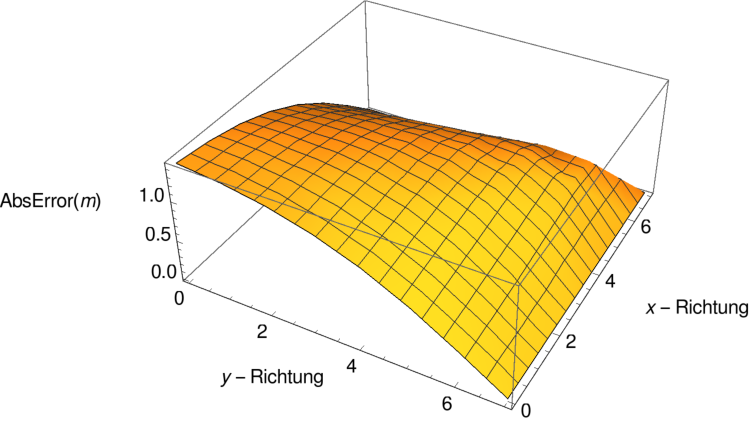
\includegraphics[width=1\linewidth]{abbildungen/vergleich_euklid_fast_marching/3DVergleich/cellsize2/Error.pdf}
\end{minipage}%
\\
\begin{minipage}{.8\textwidth}
\centering
  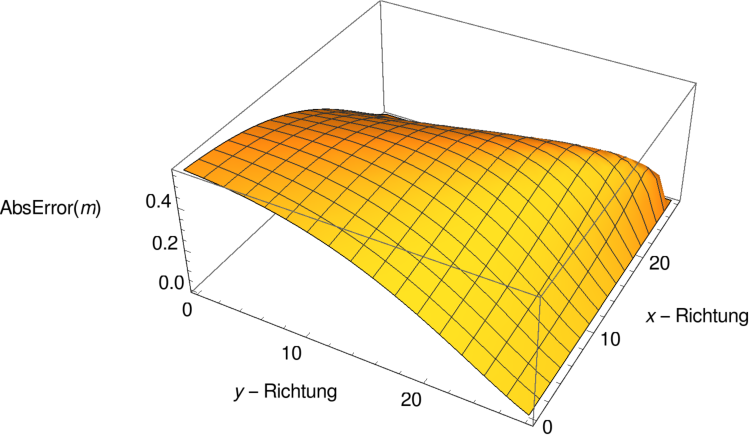
\includegraphics[width=1\linewidth]{abbildungen/vergleich_euklid_fast_marching/3DVergleich/cellsize0_5/Error.pdf}
\end{minipage}
\\
\begin{minipage}{.8\textwidth}
\centering
  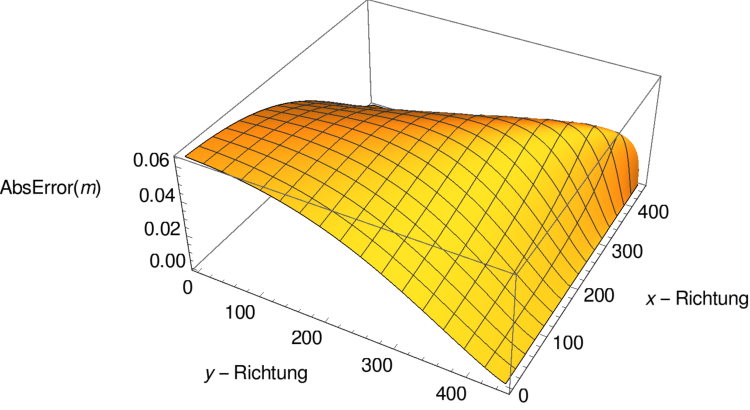
\includegraphics[width=1\linewidth]{abbildungen/vergleich_euklid_fast_marching/3DVergleich/cellsize0_03125/Error.pdf}
\end{minipage}
\caption{Darstellung des absoluten Fehlers in allen Punkten der Karte. X und Y stellen die Zellkoordinaten dar (Ohne Einheit). Zellgrößen 2 m (oben), 0,5 m (mitte) und 0,03125 m (unten)}
\label{fig_error_3d_aufstellung}
\end{figure}





\begin{figure}
\centering
\begin{minipage}{.44\textwidth}
\centering
  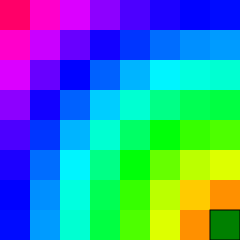
\includegraphics[width=0.9\linewidth]{abbildungen/vergleich_euklid_fast_marching/eEuclid_2m.png}
\end{minipage}%
\begin{minipage}{.44\textwidth}
\centering
  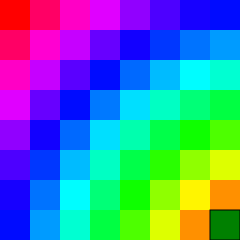
\includegraphics[width=0.9\linewidth]{abbildungen/vergleich_euklid_fast_marching/eFastMarching_2m.png}
\end{minipage}
\begin{minipage}{.1\textwidth}
\centering
  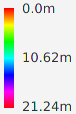
\includegraphics[width=\linewidth]{abbildungen/vergleich_euklid_fast_marching/farbskala.png}
\end{minipage}
\caption{Berechnung der Abstände mittels Euklid (links) und Fast Marching (rechts) an einem Feld mit einer Zellbreite von 2 m. Dunkelgrün: Ziel, Rot: am weitesten entfernter Punkt im Feld}
\label{fig_euklid_fast_marching_2m_cellsize}
\end{figure}



\begin{figure}[ht]
	\centering
  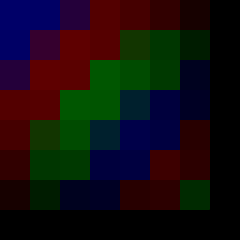
\includegraphics[width=0.4\textwidth]{abbildungen/vergleich_euklid_fast_marching/differenz_euklid_fast_marching.png}
	\caption{Differenzbildung der beiden Karten Euklid und Fast Marching bei einer Zellbreite von 2 m}
	\label{fig_fast_marching_euclid_difference}
\end{figure}




\begin{figure}
\centering
\begin{minipage}{1\textwidth}
\centering
  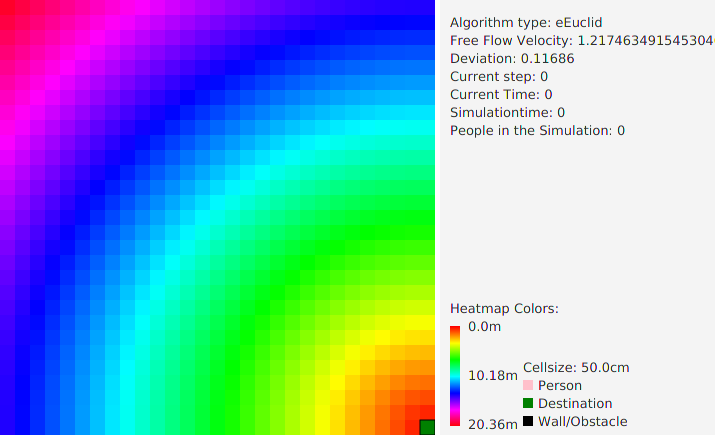
\includegraphics[width=1\linewidth]{abbildungen/vergleich_euklid_fast_marching/eEuclid_0_05m.png}
\end{minipage}%
\\
\begin{minipage}{1\textwidth}
\centering
  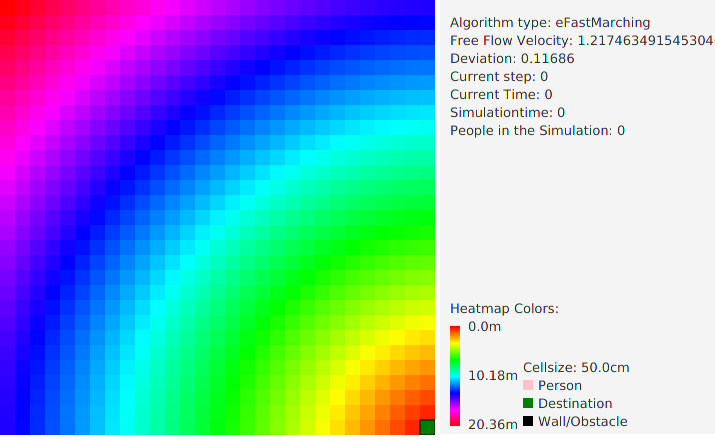
\includegraphics[width=\linewidth]{abbildungen/vergleich_euklid_fast_marching/eFastMarching_0_05m.png}
\end{minipage}
\caption{Berechnung der Abstände mittels Euklid (oben) und Fast Marching (unten) an einem Feld mit einer Zellbreite von 0,5\ m}
\label{fig_euklid_fast_marching_0_05m_cellsize}
\end{figure}

\begin{figure}[htpb]
	\centering
  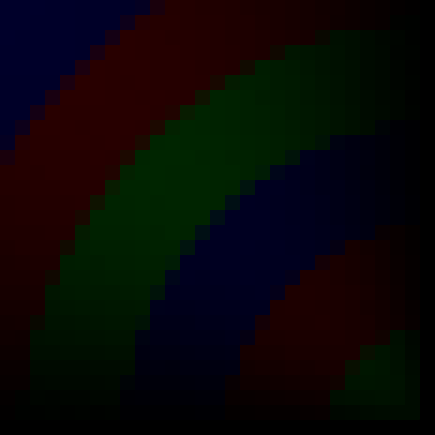
\includegraphics[width=0.6\textwidth]{abbildungen/vergleich_euklid_fast_marching/differenz_euklid_fm_0_05m.png}
	\caption{Differenzbildung der beiden Karten Euklid und Fast Marching bei einer Zellbreite von 0.5 m}
	\label{fig_fast_marching_euclid_difference_0_05m}
\end{figure}



\begin{table}[htbp]
\begin{tabular}{|l|r|r|r|r|r|r|r|}
\hline
Cellsize [m] & 2 & 1 & 0,5 & 0,25 & 0,125 & 0,0625 & 0,03125 \\ \hline
Cells in X and Y & 7 & 14 & 28 & 56 & 112 & 224 & 448 \\ \hline
Distance in  & & &  & &  & &\\ X and Y [m] & \textbf{14} & \textbf{14} & \textbf{14} & \textbf{14} & \textbf{14} & \textbf{14} & \textbf{14} \\ \hline
Tatsächliche & & &  & &  & &\\Entfernung [m] & 19,799 & 19,799 & 19,799 & 19,799 & 19,799 & 19,799 & 19,799 \\ \hline
Euklid [m] & 19,799 & 19,799 & 19,799 & 19,799 & 19,799 & 19,799 & 19,799 \\ \hline
Fast  & & &  & &  & &\\ Marching [m] & \textbf{21,245} & \textbf{20,717} & \textbf{20,363} & \textbf{20,137} & \textbf{19,997} & \textbf{19,913} & \textbf{19,863} \\ \hline
Diff [m] & 1,45 & 0,92 & 0,5645 & 0,3380 & 0,1979 & 0,1138 & 0,0644 \\ \hline
 & \multicolumn{1}{l|}{} & \multicolumn{1}{l|}{} & \multicolumn{1}{l|}{} & \multicolumn{1}{l|}{} & \multicolumn{1}{l|}{} & \multicolumn{1}{l|}{} & \multicolumn{1}{l|}{} \\ \hline
Error [\%]  & & &  & &  & &\\ diff/distance & \textbf{7,30} & \textbf{4,64} & \textbf{2,85} & \textbf{1,71} & \textbf{1,00} & \textbf{0,57} & \textbf{0,33} \\ \hline
\end{tabular}
\caption{Vergleich der Algorithmen Fast Marching und Euklid. Cellsize ist die Kantenlänge einer quadratischen Zelle in m (Zellbreite)}
\label{tab_euklid_fm_vergleich}
\end{table}


\begin{figure}[ht]
	\centering
  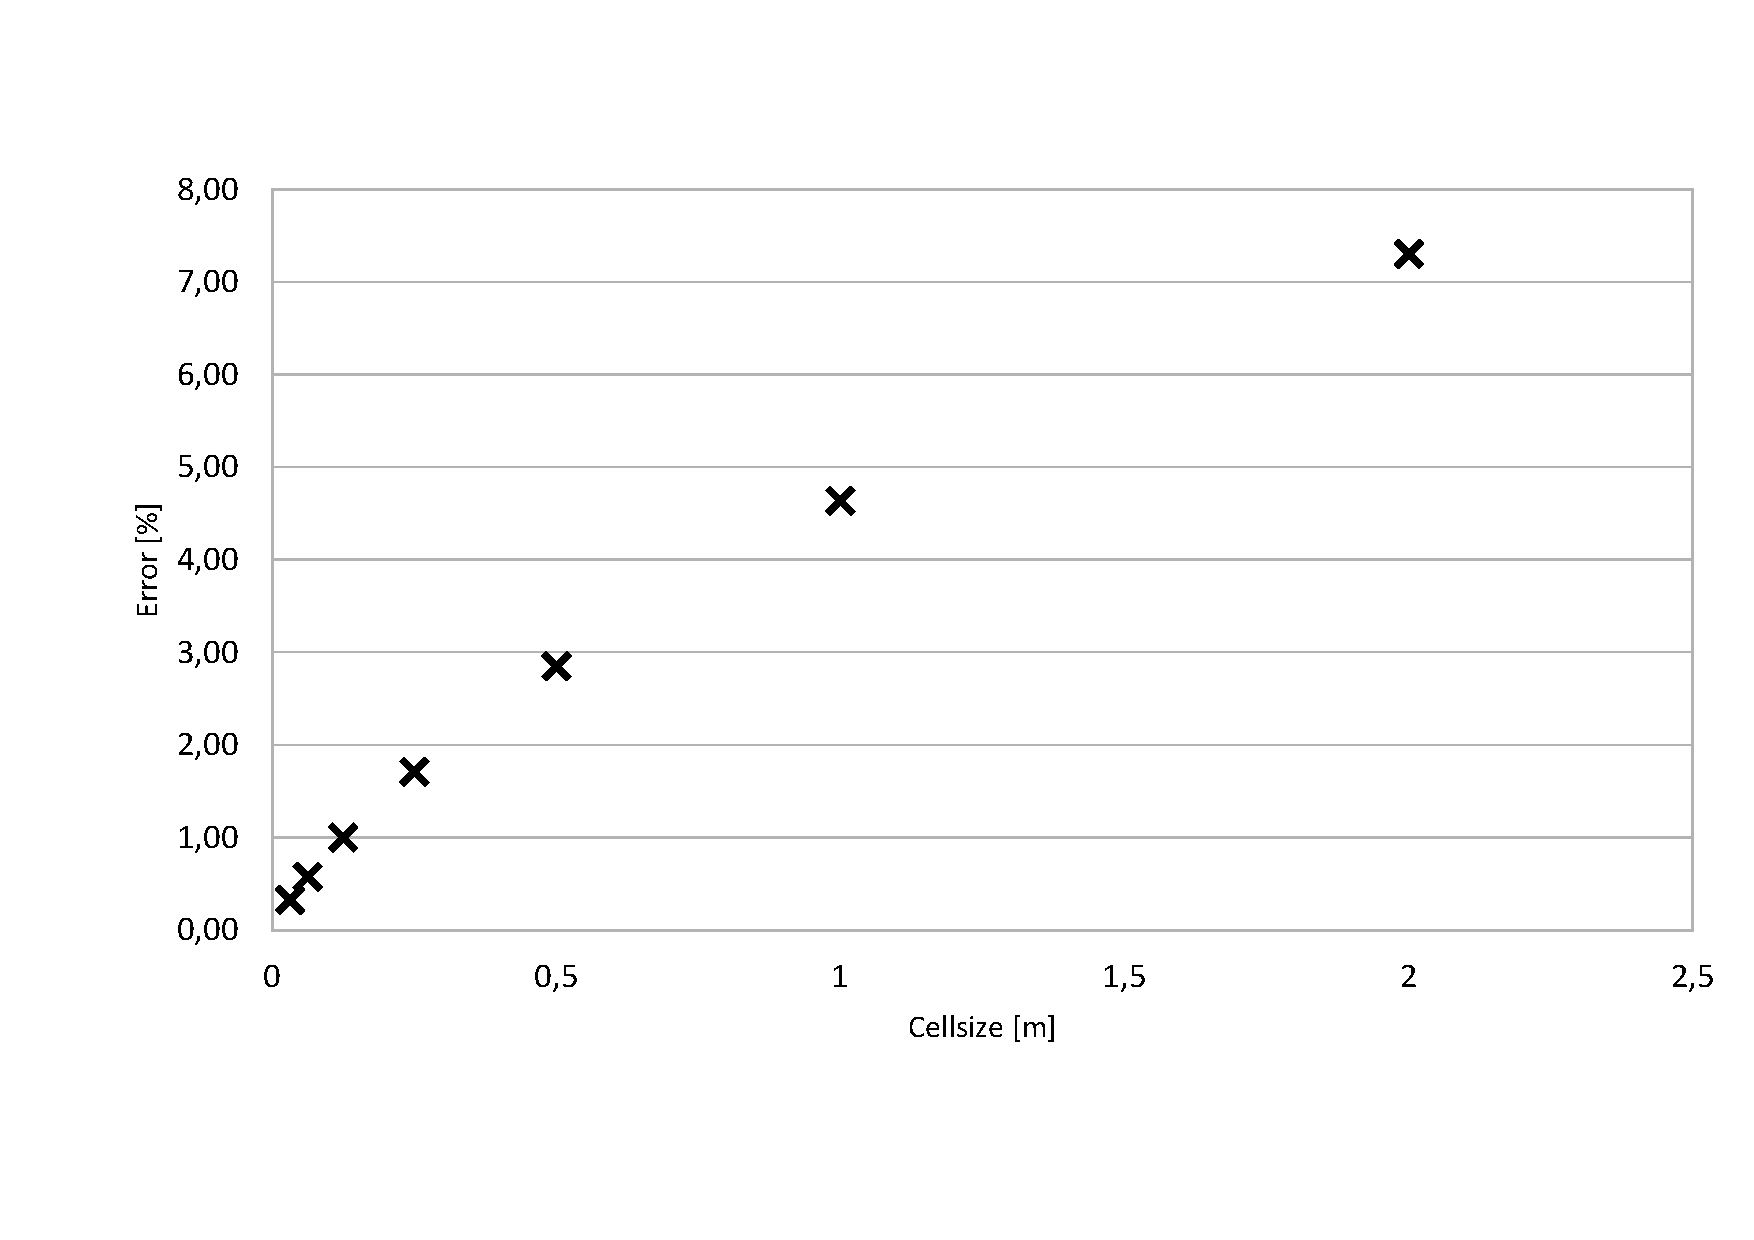
\includegraphics[width=\textwidth]{abbildungen/vergleich_euklid_fast_marching/EuklidFastMarchingError.pdf}
	\caption{Prozentualer Fehler für die diagonale Entfernung des Fast Marching Algorithmus in Abhängigkeit der Zellbreite.}
	\label{fig_fast_marching_error_cellsize}
\end{figure}


